% Chapter Template

\chapter{The Receiver} % Main chapter title

\label{Chapter5}

\section{Introduction}
The receiver for the sound-based move tracking protocol is in charge of decoding a sequence of face turns from the transmitted audio.

To do this, the receiver must go through the following steps:
\begin{enumerate}
    \item Record the transmitted audio.
    \item Measure the audible frequencies at each time step.
    \item Convert each time step's audible frequencies to the cube's state at that moment.
    \item Decode the applied face turns from the sequence of cube states.
\end{enumerate}

This chapter will describe the development of a software algorithm in Python that can serve as a receiver for this sound-based move tracking protocol. 
This development began with the creation of synthetic audio recordings representing the tones that would be emitted by a Rubik's Cube equipped with an ideal transmitter (Section \ref{sec:synthetic-audio-generation}) followed by the implementation of an algorithm capable of decoding that ideal synthetic audio (Section \ref{sec:decoding-synthetic-audio}).
The algorithm was then made more robust by adding realistic noise to the synthetic audio to better simulate a real speedcubing environment (Section \ref{sec:adding-realistic-noise}) followed by enhancing the previously designed algorithm to continue to decode the applied move sequence in the midst of the added noise (Section: \ref{sec:decoding-realistic-noise}). \footnote{The contents of this Chapter have been specially written so that the reader can copy them into a Jupyter Notebook running a Python 3.9 kernel and see the same results for himself/herself.} 


\section{Synthetic Audio Generation}
\label{sec:synthetic-audio-generation}
The first step of designing a receiver is to synthesize an audio signal representative of the output of the ideal receiver.

This is done by encoding the frequency corresponding to each centerpiece state (Section \ref{subsec:represent-audio-protocol}), creating a virtual Rubik's Cube (Section \ref{subsec:represent-rubiks-cube}), and finally generating the audio signal from the virtual Rubik's Cube's state (Section \ref{subsec:generate-audible-algorithm}).
\newpage
\subsection{Representing the Audio Protocol}
\label{subsec:represent-audio-protocol}
For the synthetic audio generator to produce a realistic signal, it needs to know which frequencies to transmit for each centerpiece state. 
For this design the frequencies listed in Table \ref{table:centerpiece-frequencies} are converted to a dictionary.

\begin{verbatim}
CENTERPIECE_ROTATION_TO_FREQUENCY_MAPPINGS = {
    "U": {
        0: 800,
        1: 900,
        2: 1000,
        3: 1100,
    },
    "D": {
        0: 1300,
        1: 1400,
        2: 1500,
        3: 1600,
    },
    "R": {
        0: 1800,
        1: 1900,
        2: 2000,
        3: 2100,
    },
    "L": {
        0: 2300,
        1: 2400,
        2: 2500,
        3: 2600,
    },
    "F": {
        0: 2800,
        1: 2900,
        2: 3000,
        3: 3100,
    },
    "B": {
        0: 3300,
        1: 3400,
        2: 3500,
        3: 3600,
    }
}
\end{verbatim}

\newpage
With this dictionary in place, determining the frequency to transmit for any particular centerpiece's current rotation is reduced to a simple lookup.
\begin{verbatim}
def frequency_of(centerpiece: str, rotation: int) -> float:
    return CENTERPIECE_ROTATION_TO_FREQUENCY_MAPPINGS[centerpiece][rotation]
\end{verbatim}

\subsection{Representing the Rubik's Cube}
\label{subsec:represent-rubiks-cube}
Next, the synthetic audio generator needs a representation of a Rubik's Cube on which face turns can be virtually applied, and the resulting cube state can be read out.
\begin{verbatim}
class RubiksCube:
    
    CLOCKWISE = 1
    COUNTERCLOCKWISE = 3

    def __init__(self):
        self.state = { "U": 0, "D": 0, "R": 0, "L": 0, "F": 0, "B": 0 }
    
    def apply_move(self, move: str):
        # Extract the face and direction from the move string.
        face = move[0]
        if len(move) == 1:                             # e.g. U
            direction = RubiksCube.CLOCKWISE
        else:                                          # e.g. U'
            direction = RubiksCube.COUNTERCLOCKWISE
        # Update the state to apply the move.
        self.state[face] = (self.state[face] + direction) % 4
\end{verbatim}

\subsection{Generating Synthetic Audio for an Arbitrary Algorithm}
\label{subsec:generate-audible-algorithm}
Now the synthetic audio can be generated for any valid algorithm.
This is done using the "tones" library \cite{pip-tones} created by Erik Nyquist.
First, a separate audio track is created for each centerpiece on the cube and the frequencies representing the initial state of each centerpiece are added to its corresponding audio track.
From there, the rest of the synthetic audio can be created by iterating through each step of the given algorithm, applying it to the virtual Rubik's Cube, and adding the frequency for each centerpiece's resulting state to its corresponding audio track.

\begin{verbatim}
from tones.mixer import Mixer  # https://pypi.org/project/tones/
from tones import SINE_WAVE
    
def _create_mixer(rubiks_cube: RubiksCube) -> Mixer:
    mixer: Mixer = Mixer(sample_rate=44100, amplitude=1)
    # Add a separate track for each centerpiece.
    for face, _ in rubiks_cube.state.items():
        mixer.create_track(face, SINE_WAVE, attack=0, decay=0)
    return mixer

def _render_cube_state(mixer: Mixer, rubiks_cube: RubiksCube, tps: float):
    for face, rotation in rubiks_cube.state.items():
        mixer.add_tone(face, frequency_of(face, rotation), duration=1 / tps)

def render_audible_alg(alg: str, wav_path: str=None, tps: float=4):
    # Create the virtual Rubik's Cube.
    rubiks_cube: RubiksCube = RubiksCube()
    
    # Create the audio mixer used to create the synthesized audio.
    mixer = _create_mixer(rubiks_cube)
    
    # Add the initial cube state to the mixer.
    _render_cube_state(mixer, rubiks_cube, tps)
    
    # Iterate over the moves in the algorithm, adding
    # the cube state to the mixer after each move.
    moves = alg.split(" ")
    for move in moves:
        rubiks_cube.apply_move(move)
        _render_cube_state(mixer, rubiks_cube, tps)
    
    # Save the final audio to a .wav file.
    mixer.write_wav(wav_path if wav_path else f"{alg}.wav")
\end{verbatim}

With these functions in place, synthetic audio can be easily created for any valid Rubik's Cube algorithm. For example, generating synthetic audio that sweeps through every possible centerpiece state can be done with the following snippet of code:

\begin{verbatim}
demo_alg = "U U U U D D D D R R R R L L L L F F F F B B B B"
demo_wav_path = "demo_all_states.wav"
render_audible_alg(demo_alg, demo_wav_path)
\end{verbatim}


\section{Decoding Move Sequences from Synthetic Audio}
\label{sec:decoding-synthetic-audio}
With synthetic audio now available for any valid Rubik's Cube algorithm, the next step is to create an initial software algorithm that can decode that audio back into the original move sequence.

Accomplishing this will require computing the synthetic audio's spectrogram (Section \ref{subsec:compute-spectrogram}), followed by extracting the dominant frequencies present at each time step (Section \ref{subsec:extract-dominant-freqs}), and converting those dominant frequencies into the corresponding Rubik's Cube centerpiece states (Section \ref{subsec:translating-freqs-to-state}), all before finally recovering the originally applied move sequence (Section \ref{subsec:extract-moves}).

\newpage
\subsection{Compute the Spectrogram}
\label{subsec:compute-spectrogram}
The first step in decoding the synthetic audio is determining its component frequencies at any specific moment in time.
These component frequencies can be easily visualized using a spectrogram, like the one in Figure \ref{fig:spectrogram} of the synthetic audio created in Section \ref{subsec:generate-audible-algorithm}.

\begin{figure}[h]
    \centering
    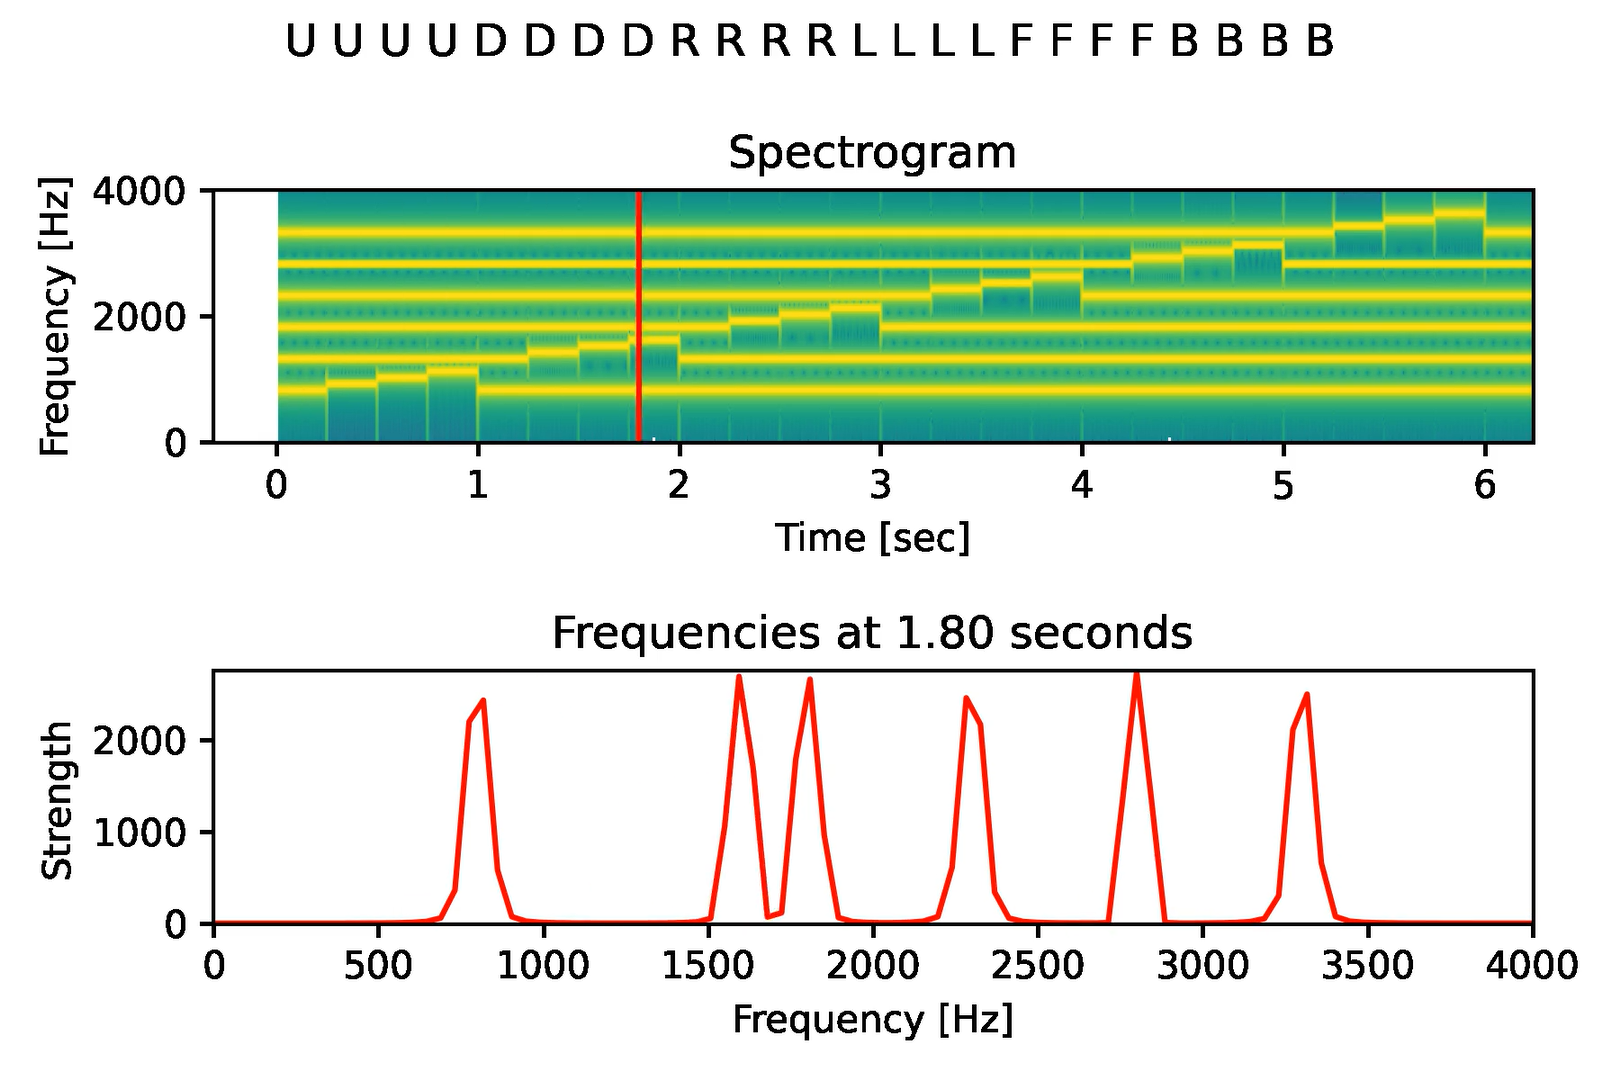
\includegraphics[width=0.8\textwidth]{Figures/5 Algorithm Design/component_frequencies.png}
    \caption{Spectrogram of the synthetic audio created in Section \ref{subsec:generate-audible-algorithm}. The source code for this diagram is available in Appendix \ref{sec:code-spectrogram}.}
    \label{fig:spectrogram}
\end{figure}

The bright, horizontal yellow bands in the spectrogram represent the component frequencies present in the audio signal at each point in time.
The vertical red line on the spectrogram indicates the specific slice of the spectrogram represented by the graph of the component frequencies at that specific point in time.

While the Figure \ref{fig:spectrogram} was created using Matplotlib's specgram plot, the actual data of the spectrogram for a given .wav file can be easily obtained using the numpy and scipy packages

\begin{verbatim}
import numpy as np
from scipy import signal
from scipy.io import wavfile

def compute_spectrogram(wav_path: str):
    SAMPLES_PER_WINDOW = 1024  # Balances frequency/time precision
    sample_rate, audio_samples = wavfile.read(wav_path)
    freq, time, Zxx = signal.stft(audio_samples, fs=sample_rate,
        nperseg=SAMPLES_PER_WINDOW, noverlap=(SAMPLES_PER_WINDOW // 4) * 3)
    spectrogram = np.abs(Zxx).transpose()
    return freq, time, spectrogram
\end{verbatim}

\newpage
\subsection{Extract the Dominant Component Frequencies}
\label{subsec:extract-dominant-freqs}
Notice how the component frequency graph in Figure \ref{fig:spectrogram} has six peaks: these are the transmitted frequencies representing the current state of the virtual Rubik's Cube's six centerpieces at that specific instant of time.

The exact frequencies of these peaks can be extracted by filtering out all frequencies not above a specific threshold.
In this case, a simple threshold of 85\% of the maximum strength of any component frequency (see the green line in Figure \ref{fig:spectrogram-with-naive-threshold}) isolates the peak of the six dominant component frequencies.

\begin{figure}[h]
    \centering
    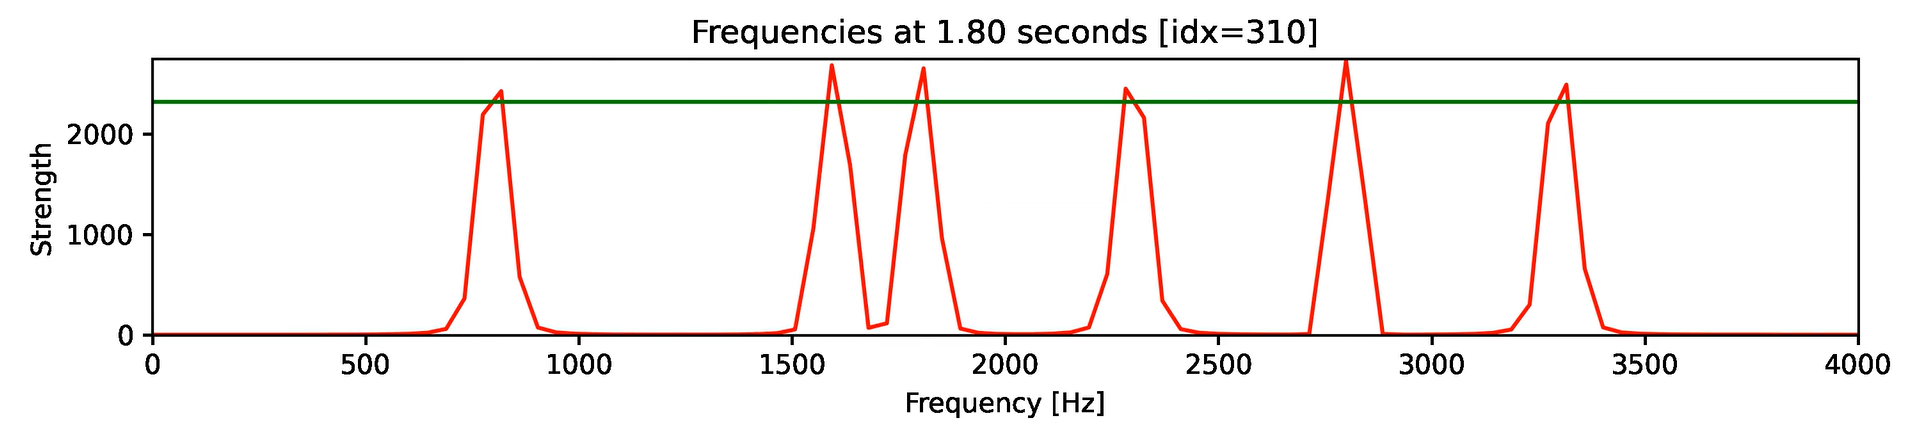
\includegraphics[width=0.8\textwidth]{Figures/5 Algorithm Design/threshold.png}
    \caption{Spectrogram of the synthetic audio created in Section \ref{subsec:generate-audible-algorithm} with a threshold at 85\% of the maximum strength of the component frequencies. The source code for this diagram is available in Appendix \ref{sec:code-spectrogram-with-naive-threshold}.}
    \label{fig:spectrogram-with-naive-threshold}
\end{figure}

Using the actual spectrogram data we can compute the exact values of these peaks.
\begin{verbatim}
def compute_threshold(values: list):
    return max(values) * 0.85

def extract_important_frequencies(freq, time, spectrogram, time_idx):
    important_freqs = []
    threshold = compute_threshold(spectrogram[time_idx])
    for freq_idx in range(len(freq)):
        if spectrogram[time_idx][freq_idx] > threshold:
            important_freqs.append(dict(
                hz=freq[freq_idx],
                power=spectrogram[time_idx][freq_idx]
            ))
    return important_freqs

freq, time, spectrogram = compute_spectrogram(demo_wav_path)
important_freqs = extract_important_frequencies(freq, time, spectrogram,
    time_idx=310) # 1.80 seconds

important_freqs_hz = [i["hz"] for i in important_freqs]
pretty_freqs = list(map(lambda x: f"{x:.0f} Hz", important_freqs_hz))
print(pretty_freqs)

>> ["818 Hz", "1593 Hz", "1809 Hz", "2283 Hz", "2799 Hz", "3316 Hz"]
\end{verbatim}

\newpage
\subsection{Translating Component Frequencies to Centerpiece States}
\label{subsec:translating-freqs-to-state}
With the specific frequencies of each detected peak, the original state of the Rubik's Cube at that moment in time can be computed by finding the state whose corresponding frequency is closest to each detected peak frequency.

\begin{verbatim}
def _closest_state(detected_freq):
    closest_rotation = None
    closest_difference = None
    for face, rotations in CENTERPIECE_ROTATION_TO_FREQUENCY_MAPPINGS.items():
        for rotation, freq in rotations.items():
            difference = abs(detected_freq - freq)
            if closest_difference is None or difference < closest_difference:
                closest_difference = difference
                closest_rotation = dict(face=face, rotation=rotation)
    return closest_rotation

def get_state_from_freqs(important_freqs: list) -> dict:
    state = {}
    for freq in important_freqs:
        hz, power = freq.values()
        closest_state = _closest_state(hz)
        state[closest_state['face']] = closest_state['rotation']
    return state

print(get_state_from_freqs(important_freqs))

>> {"U": 0, "D": 3, "R": 0, "L": 0, "F": 0, "B": 0}
\end{verbatim}

Repeating this process for each time step in the recorded audio will yield a sequence of the Rubik's Cube's centerpiece states over the course of the recorded audio sequence.

\begin{verbatim}
def get_state_over_time(freq, time, spectrogram):
    state_over_time = []
    for time_idx in range(len(time)):
        important_freqs = extract_important_frequencies(
            freq, time, spectrogram, time_idx)
        state = get_state_from_freqs(important_freqs)
        state_over_time.append(dict(
            time=time[time_idx],
            state=state
        ))
    return state_over_time

state_over_time = get_state_over_time(freq, time, spectrogram)
\end{verbatim}

\newpage
\subsection{Extracting Move Sequences from Centerpiece State Sequences}
\label{subsec:extract-moves}
Finally, the original move sequence can be recovered by iterating over the sequence of cube states, and registering any change to the cube state as a move applied to the cube.

\begin{verbatim}
def _move_from(face, current_rotation, new_rotation):
    direction = None
    if (current_rotation + RubiksCube.CLOCKWISE) % 4 == new_rotation:
        direction = ""  # Clockwise
    elif (current_rotation + RubiksCube.COUNTERCLOCKWISE) % 4 == new_rotation:
        direction = "'" # Counterclockwise
    return f"{face}{direction}"

def detect_moves(state_over_time):
    detected_moves = []
    current_state = {}
    for idx, timed_state in enumerate(state_over_time):
        time, state = timed_state.values()
        for face, rotation in state.items():
            if not (face in current_state):
                current_state[face] = rotation
            if rotation != current_state[face]:
                detected_moves.append(dict(
                    time=time,
                    move=_move_from(face, current_state[face], rotation)
                ))
                current_state[face] = rotation
    return detected_moves

detected_moves = detect_moves(state_over_time)

pretty_moves = " ".join([i["move"] for i in detected_moves])
print(pretty_moves)   
print(f"Matches demo_alg? {demo_alg == pretty_moves}") 

>> U U U U D D D D R R R R L L L L F F F F B B B B
>> Matches demo_alg? True
\end{verbatim}

Clearly, the detected move sequence matches the demo algorithm used to create the synthetic audio in Section \ref{subsec:generate-audible-algorithm}, which means this algorithm is a functional receiver for an ideal transmitter.


\newpage
\section{Adding Realistic Noise to the Synthetic Audio}
\label{sec:adding-realistic-noise}
While Section \ref{sec:decoding-synthetic-audio}'s successful recovery of a sequence of moves applied to a virtual Rubik's Cube is impressive, the synthetic audio is not realistic.
This is made obvious by a comparison between the spectrograms of the background audio in Figure \ref{fig:signal-to-noise-ratio} and the synthetic audio in Figure \ref{fig:spectrogram}.
In the latter, the bright yellow indicators of present frequencies are very clear and strong with no other frequencies present in the signal.
In contrast, the former contains many areas with bright pink indicators of prominent frequencies (the color differences are due to the use of different applications to generate the diagrams).
A more realistic signal would contain both the strong bands of the transmitted frequency along with the underlying background noise of whatever cube is actively being solved.

Adding this noise could be done in software by overlaying the synthetic audio with a recording of the background noise, but it was just as easy to play the synthetic audio from a laptop speaker and record it using a nearby smartphone while solving various Rubik's Cubes.
An example of the resulting spectrogram can be seen in Figure \ref{fig:noisy-spectrogram}.
\footnote{The astute reader will notice that the audio bands in Figure \ref{fig:noisy-spectrogram} fall on different frequencies than in Figure \ref{fig:spectrogram}. This is because the realistic audio samples encoded centerpiece states using slightly different frequency assignments than the synthetic audio generated in Section \ref{sec:synthetic-audio-generation}.}

\begin{figure}[h]
    \centering
    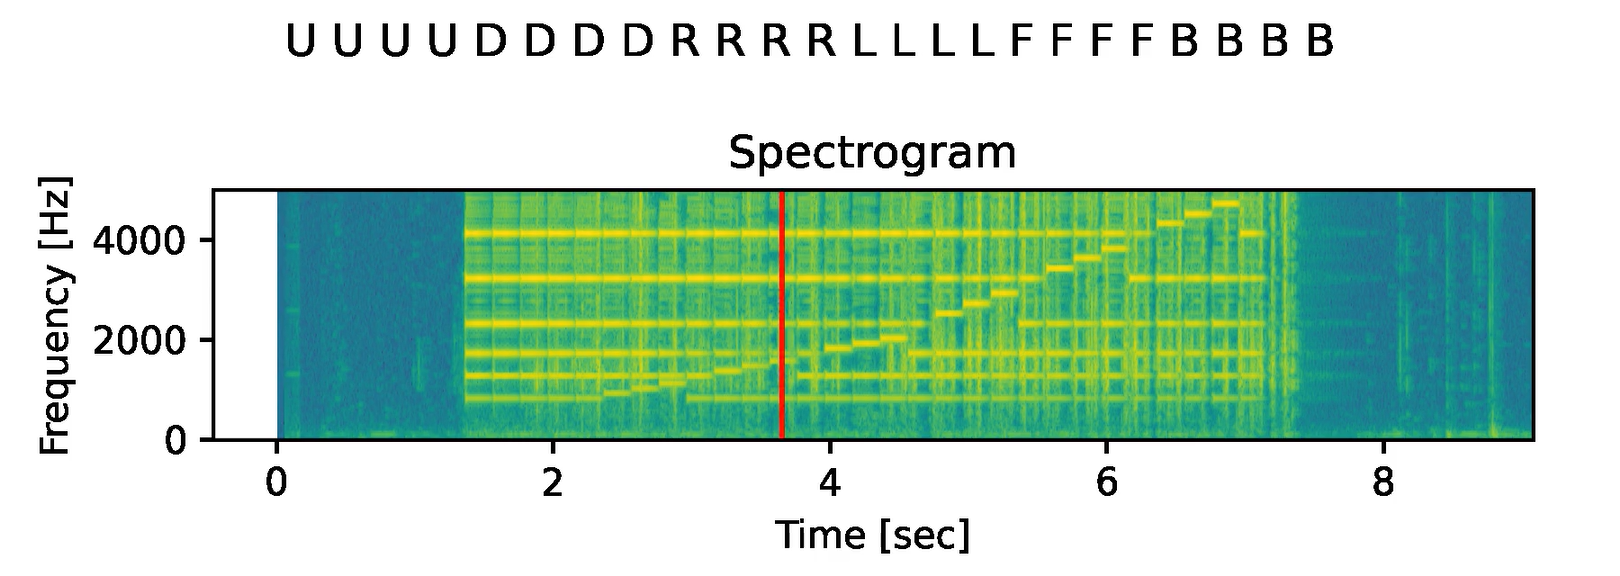
\includegraphics[width=0.8\linewidth]{Figures/5 Algorithm Design/transmitted-356-5tps.png}
    \caption{A spectrogram of the audio representing the demo algorithm from Section \ref{subsec:generate-audible-algorithm} as recorded by a Google Pixel smartphone while actively solving a Gans 356 speedcube.}
    \label{fig:noisy-spectrogram}
\end{figure}

Notice how the horizontal bands representing the transmitted signal are dimmer in the realistic audio.
This reflects the loss of volume any sound experiences as it travels through the air.
Additionally, the transmitted signal is also partially obscured by the additional audible noise of the Rubik's Cube's turns.

\section{Decoding Move Sequences from Realistic Audio}
\label{sec:decoding-realistic-noise}
The loss of signal strength alongside the added noise creates several unique challenges that require more sophisticated analysis than that presented in Section \ref{sec:decoding-synthetic-audio}.

\subsection{Fine-Tuning the Threshold}
\label{subsec:fine-tuning-threshold}
Because some audio frequencies are dampened more than others as they travel through the air to the recording microphone, a static threshold like the one used in Section \ref{subsec:extract-dominant-freqs} fails to capture all the dominant frequencies that compose the audible signal (See Figure \ref{fig:threshold-miss})

\begin{figure}[h]
    \centering
    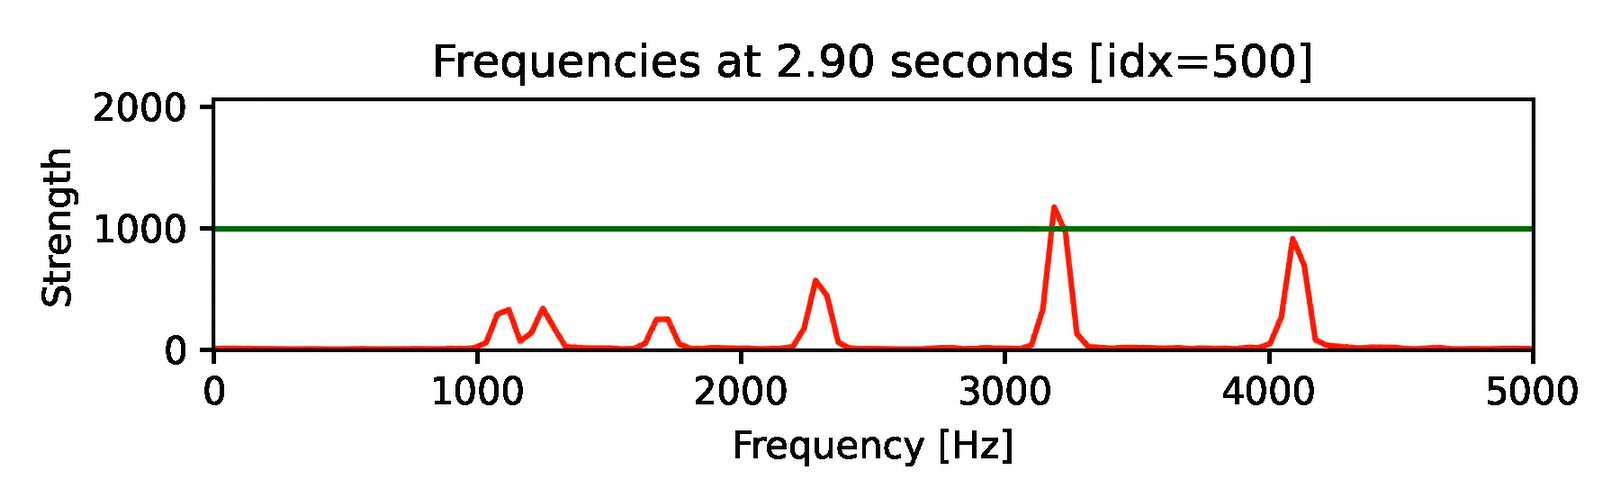
\includegraphics[width=0.8\linewidth]{Figures/5 Algorithm Design/threshold-miss.png}
    \caption{The 85\% threshold from Section \ref{subsec:extract-dominant-freqs} misses most of the signal peaks when applied to realistic audio}
    \label{fig:threshold-miss}
\end{figure}

Furthermore, the natural background noise can also cause false positives during the moments between moves while the signal is weaker as a result of changing from one state to the next (See Figure \ref{fig:threshold-false-positives}).

\begin{figure}[h]
    \centering
    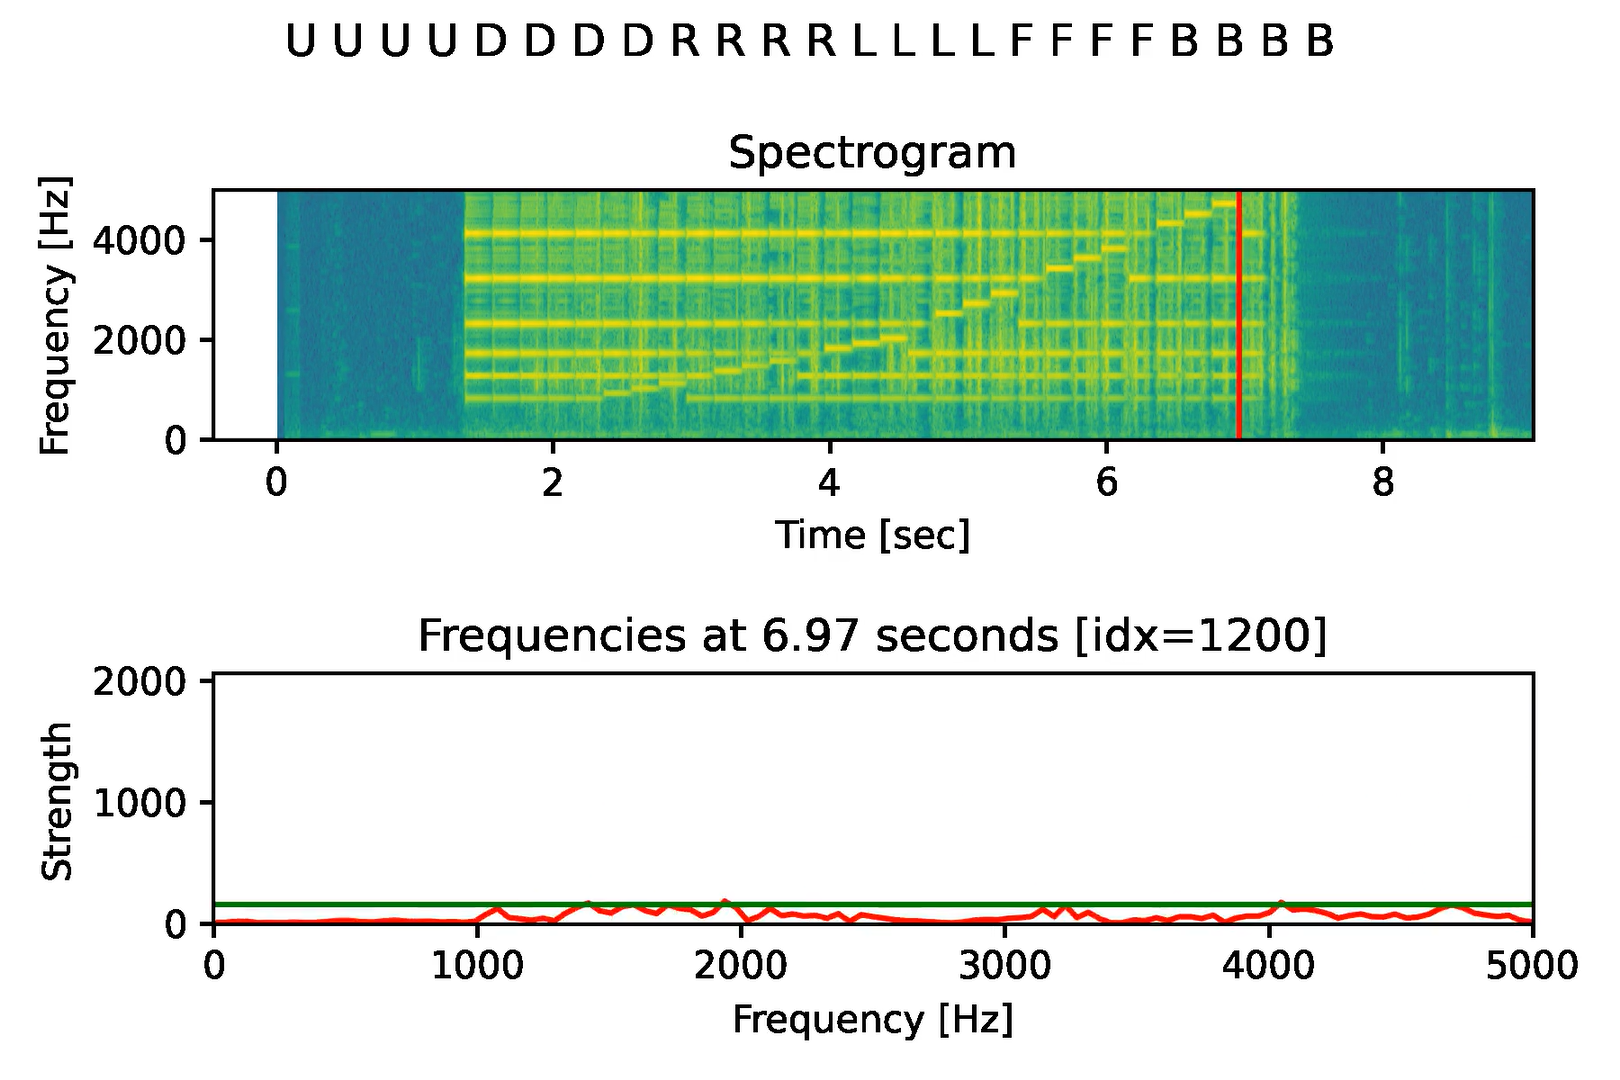
\includegraphics[width=0.8\linewidth]{Figures/5 Algorithm Design/threshold-false-positives.png}
    \caption{Between face turns, when the audio signal is nearly non-existent, the background noise can falsely register the presence of random centerpiece states}
    \label{fig:threshold-false-positives}
\end{figure}

Fortunately, since the power of the peak frequencies which contain the audio signal are generally statistical outliers among the set of component frequencies basing the threshold at one standard deviation above the mean generally captures all the peak frequencies while still excluding the underlying noise of the cube/environment. Additionally, the use of a hard minimum value for the threshold helps reduce the number of false positives during the gaps in the signal between face turns. (See Figure \ref{fig:threshold-refined})
\begin{verbatim}
def compute_threshold(values: list, stdv_pct: float=1, min_thresh: int=50):
    return max(min_thresh, np.std(values) * stdv_pct)
\end{verbatim}

\begin{figure}[h]
    \centering
    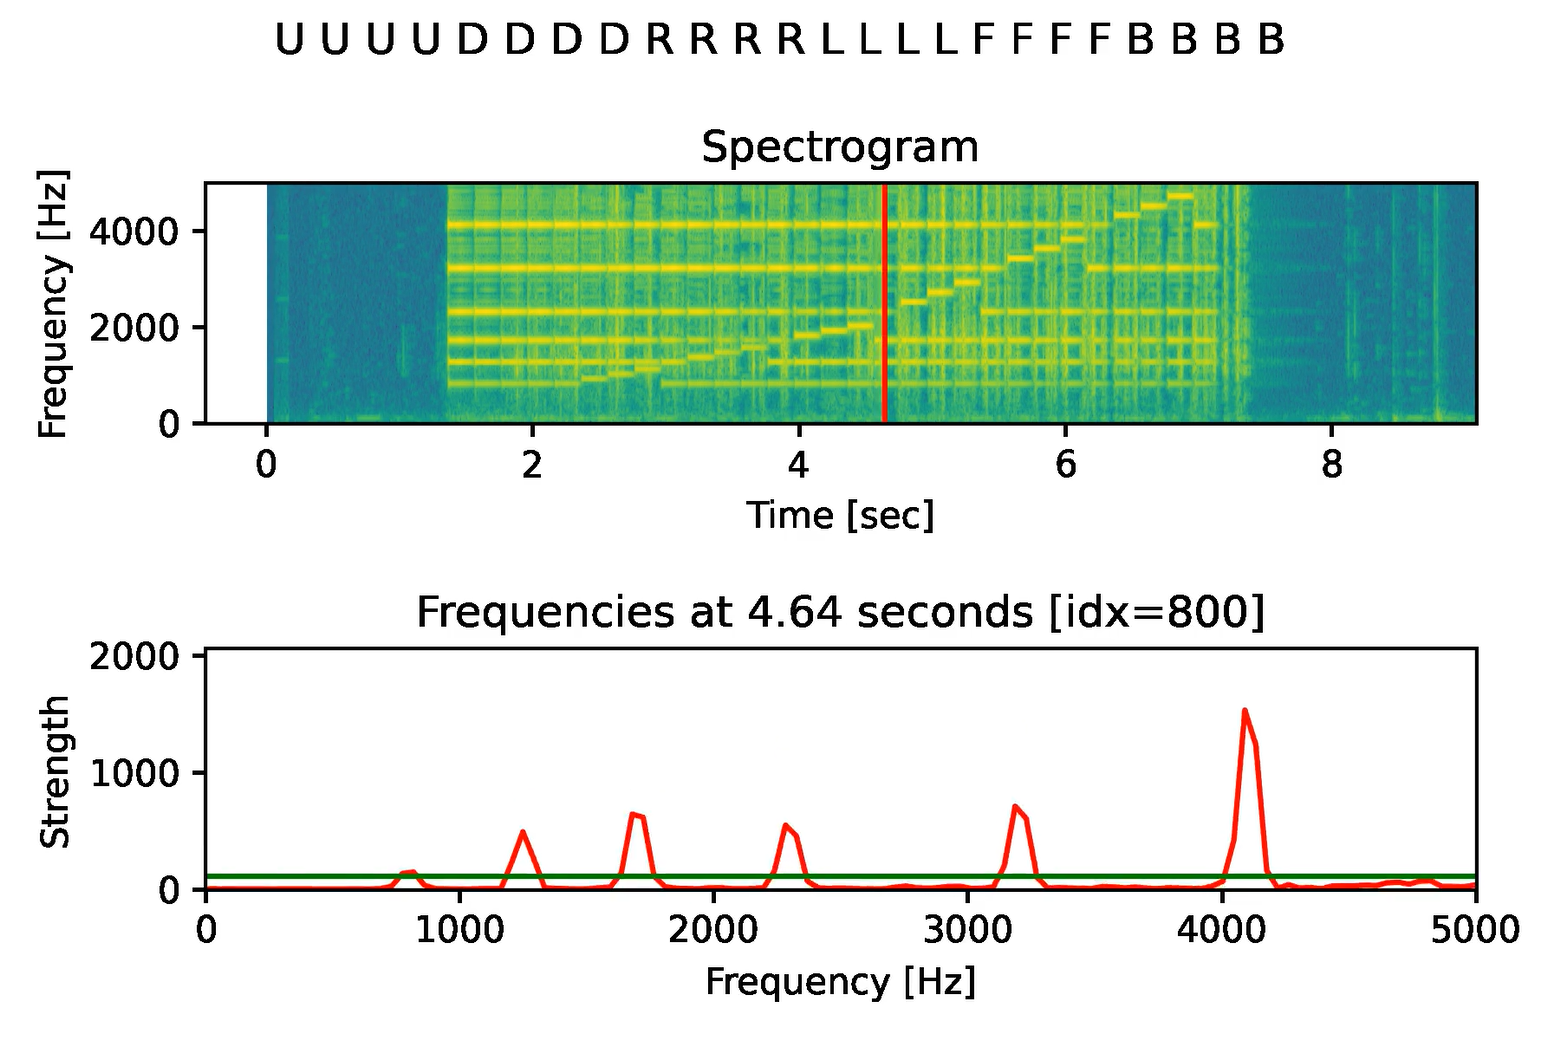
\includegraphics[width=0.8\linewidth]{Figures/5 Algorithm Design/threshold-refined.png}
    \caption{Tying the threshold to the standard deviation of the power of the component frequencies at a specific time step consistently captures all the peak frequencies.}
    \label{fig:threshold-refined}
\end{figure}

\subsection{Filtering through Similar Peak Frequencies}
\label{subsec:filtering-similar-peak-frequencies}
While the new threshold calculation does properly capture all the peak frequencies, it also captures more samples than just the six tips of each peak. 
These extra samples can cause confusion when trying to extract each centerpiece's state if they correspond to different states for the same centerpiece.
That said, as long as the power of each frequency is also saved, then any disagreements about a specific centerpiece's state can be resolved by accepting the one with the most intense frequency as the actual state.

\begin{verbatim}
def get_state_from_freqs(important_freqs: list) -> dict:
    state = {}
    state_power = {"U": 0, "D": 0, "R": 0, "L": 0, "F": 0, "B": 0}  # New
    for freq in important_freqs:
        hz, power = freq.values()
        closest_state = _closest_state(hz)
        if power > state_power[closest_state["face"]]:              # New
            state[closest_state["face"]] = closest_state["rotation"]
            state_power[closest_state["face"]] = power              # New
    return state

transmitted_wav_path = "transmitted-356-5tps.wav"
freq, time, spectrogram = compute_spectrogram(transmitted_wav_path)
important_freqs = extract_important_frequencies(freq, time, spectrogram,
    time_idx=800) # 4.64 seconds
print(get_state_from_freqs(important_freqs))

>> {"U": 0, "D": 0, "R": 0, "L": 0, "F": 0, "B": 0}
\end{verbatim}

\newpage
\subsection{Ignoring Noise when Extracting Move Sequences}
\label{subsec:ignoring-noise-when-extracting-move-sequences}
However, the background noise occasionally causes the detection of an incorrect centerpiece state despite these noise filtering measures.
Since the approach in Section \ref{subsec:extract-moves} registers an applied face turn for \emph{any} detected change in a centerpiece's state, \emph{any} mis-detection would incorrectly register a face turn that never happened.

Fortunately, this issue can be mitigating by adding a simple sliding window to ensure that the state change persists over several time steps instead of blindly accepting any detected change in a centerpiece's state as a new face turn.

\begin{verbatim}
def detect_moves(state_over_time, window_size=8):                       # Edit
    detected_moves = []
    current_state = {}
    new_state = {"U": -1, "D": -1, "R": -1, "L": -1, "F": -1, "B": -1}  # New
    new_state_idx = {"U": 0, "D": 0, "R": 0, "L": 0, "F": 0, "B": 0}    # New
    for idx, timed_state in enumerate(state_over_time):
        time, state = timed_state.values()
        for face, rotation in state.items():
            # Update new_state whenever the rotation changes
            if rotation != new_state[face]:
                new_state[face] = rotation
                new_state_idx[face] = idx
            # If the new state has persisted over window_size time steps...
            if idx - new_state_idx[face] == window_size:
                if not (face in current_state):
                    current_state[face] = new_state[face]
                # ... and it's a different rotation than the current state...
                elif new_state[face] != current_state[face]:
                    # ... then we have detected a face turn!
                    detected_moves.append(dict(
                        time=state_over_time[new_state_idx[face]]["time"],
                        move=_move_from(face, current_state[face], rotation)
                    ))
                    current_state[face] = rotation
                    new_state_idx[face] = 0
    return detected_moves

state_over_time = get_state_over_time(freq, time, spectrogram)
detected_moves = detect_moves(state_over_time)

pretty_moves = " ".join([i["move"] for i in detected_moves])
print(pretty_moves)   
print(f"Matches demo_alg? {demo_alg == pretty_moves}")

>> U U U U D D D D R R R R L L L L F F F F B B B B
>> Matches demo_alg? True
\end{verbatim}

\subsection{Optimizing algorithm parameters}
\label{subsec:optimizing-params}
Determining the specific values for each of the new parameters that enabled this successful move sequence detection through the realistic noise required lots of testing and fine-tuning.
While each cube responded differently to various combinations of settings, this testing discovered multiple combinations for each cube that would yield a perfect extraction of the original move sequence.

A detailed exploration of this testing and its findings is discussed in Chapter \ref{Chapter7}.
